% SPDX-FileCopyrightText: 2026 Cyprien PIERRE
% SPDX-License-Identifier: CC-BY-4.0
\documentclass[tikz,border=5pt]{standalone}
\usepackage[T1]{fontenc}
\usepackage{lmodern}
\usetikzlibrary{arrows.meta,positioning}
\begin{document}
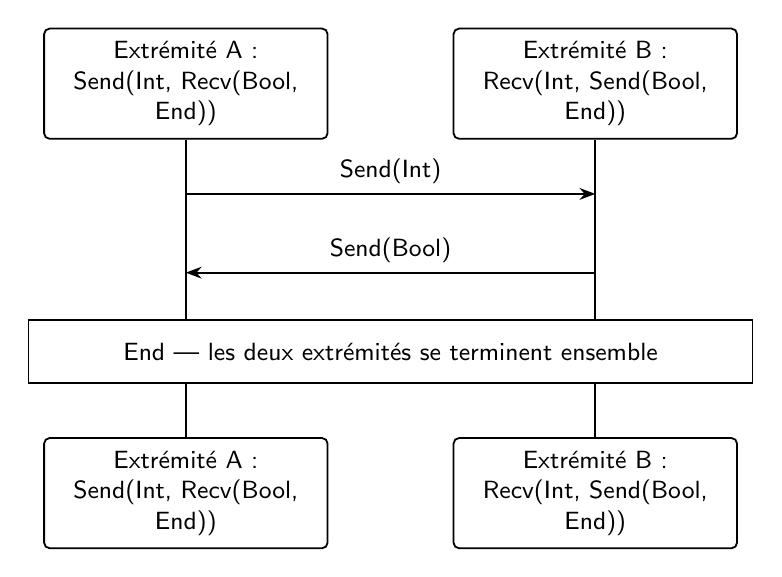
\begin{tikzpicture}[
  font=\sffamily\small,
  head/.style={draw, rounded corners=2pt, align=center, line width=.65pt, minimum height=14mm, minimum width=36mm},
  life/.style={line width=.65pt},
  message/.style={-{Stealth[length=2mm]}, line width=.7pt},
  note/.style={draw, line width=.5pt, align=center, minimum height=8mm}
]
\node[head] (a) at (0,0) {Extrémité A :\\Send(Int, Recv(Bool,\\End))};
\node[head] (b) at (52mm,0) {Extrémité B :\\Recv(Int, Send(Bool,\\End))};
\node[head] (a2) at (0,-52mm) {Extrémité A :\\Send(Int, Recv(Bool,\\End))};
\node[head] (b2) at (52mm,-52mm) {Extrémité B :\\Recv(Int, Send(Bool,\\End))};
\draw[life] (a) -- (a2);
\draw[life] (b) -- (b2);
\draw[message] (0,-14mm) -- node[above] {Send(Int)} (52mm,-14mm);
\draw[message] (52mm,-24mm) -- node[above] {Send(Bool)} (0,-24mm);
\node[note, fill=white, minimum width=92mm] at (26mm,-34mm) {End --- les deux extrémités se terminent ensemble};
\end{tikzpicture}
\end{document}
